% =====================================================================
%  Capítulo 14. Modelos de factores y valoración de activos
% =====================================================================
\chapter[Modelos de factores]{Modelos de factores: Fama-French, la prueba GRS y Fama-MacBeth}\label{cap:factores}

\section*{Objetivos de aprendizaje}
Al terminar este capítulo, el lector podrá:
\begin{enumerate}[label=\arabic*.,leftmargin=*]
  \item Estimar modelos de factores de series de tiempo (CAPM, Fama-French, Carhart) e interpretar los alfas como
        errores de valoración.
  \item Demostrar la distribución de los alfas estimados, aplicar la prueba GRS y entenderla como una comparación de
        razones de Sharpe.
  \item Estimar primas por riesgo con el método de dos pasos de Fama y MacBeth y corregir sus errores estándar
        por el problema de las variables generadas (Shanken).
  \item Extraer factores estadísticos con componentes principales y relacionarlos con los factores económicos.
\end{enumerate}

\section*{Motivación}
El Capítulo~\ref{cap:capm} estimó el CAPM activo por activo. Pero la pregunta de fondo de la valoración de activos es
conjunta: ¿explican unos pocos factores de riesgo las diferencias de rendimiento promedio entre \emph{todas} las
carteras? Desde Fama y French (1993), la respuesta estándar agrega al mercado un factor de tamaño (SMB, \emph{small
minus big}) y uno de valor (HML, \emph{high minus low} razón libro/mercado); Carhart (1997) añadió el momentum. Este
capítulo enseña a contrastar esos modelos con todas las carteras a la vez, a estimar cuánto se paga por cada riesgo y
a reconocer las trampas estadísticas de hacerlo.

\paragraph{Datos del capítulo.} Excesos de rendimiento mensuales (en porcentaje) de 30 carteras de la base de Kenneth
French: 9 formadas por tamaño y razón libro/mercado (S1V1 a S5V5, de pequeñas a grandes y de crecimiento a valor), 9
por tamaño y momentum (S1M1 a S5M5, de perdedoras a ganadoras) y 12 industrias; y los factores Mkt, SMB, HML y Mom,
de enero de 1949 a marzo de 2017 ($T=819$).

% ---------------------------------------------------------------------
\section{Regresiones de series de tiempo}
% ---------------------------------------------------------------------

Sea $\mathbf R_t$ el vector de excesos de rendimiento de $N$ carteras y $\mathbf f_t$ el de $L$ factores que también
son excesos de rendimiento de carteras (factores \emph{negociables}). Para cada cartera,
\[
  R_{it}=\alpha_i+\boldsymbol\beta_i'\mathbf f_t+\varepsilon_{it},\qquad i=1,\dots,N .
\]
Tomando esperanzas, $\E[R_i]=\alpha_i+\boldsymbol\beta_i'\E[\mathbf f]$. Un modelo de factores dice que el rendimiento
esperado se explica solo por la exposición a los factores, $\E[R_i]=\boldsymbol\beta_i'\boldsymbol\lambda$, y como un
factor negociable debe valorarse a sí mismo, $\boldsymbol\lambda=\E[\mathbf f]$. El modelo implica entonces que
\emph{todos} los alfas son cero. Un alfa es el rendimiento que el modelo no explica: un error de valoración.

\begin{proposicion}[Distribución de los alfas]\label{prop:alfas}
Si los $\boldsymbol\varepsilon_t$ son i.i.d.\ $N(\mathbf 0,\Sigma)$ e independientes de los factores, condicionado en los
factores
\[
  \hat{\boldsymbol\alpha}\sim N\Bigl(\boldsymbol\alpha,\ \frac{1}{T}\bigl(1+\hat{\boldsymbol\mu}'\hat\Omega^{-1}\hat{\boldsymbol\mu}\bigr)\Sigma\Bigr),
\]
donde $\hat{\boldsymbol\mu}$ y $\hat\Omega=\frac1T\sum_t(\mathbf f_t-\hat{\boldsymbol\mu})(\mathbf f_t-\hat{\boldsymbol\mu})'$ son la media y la
covarianza muestrales de los factores.
\end{proposicion}

\begin{proof}
En la regresión de MCO con constante, el estimador del intercepto es
$\hat\alpha_i=\bar R_i-\hat{\boldsymbol\beta}_i'\hat{\boldsymbol\mu}$. Sustituyendo $\bar R_i=\alpha_i+\boldsymbol\beta_i'\hat{\boldsymbol\mu}+\bar\varepsilon_i$
y $\hat{\boldsymbol\beta}_i=\boldsymbol\beta_i+(T\hat\Omega)^{-1}\sum_t(\mathbf f_t-\hat{\boldsymbol\mu})\varepsilon_{it}$:
\begin{align*}
  \hat\alpha_i-\alpha_i &= \bar\varepsilon_i-(\hat{\boldsymbol\beta}_i-\boldsymbol\beta_i)'\hat{\boldsymbol\mu}\\
                        &= \frac1T\sum_t\varepsilon_{it}-\hat{\boldsymbol\mu}'(T\hat\Omega)^{-1}\sum_t(\mathbf f_t-\hat{\boldsymbol\mu})\varepsilon_{it}\\
                        &= \frac1T\sum_t\Bigl[1-\hat{\boldsymbol\mu}'\hat\Omega^{-1}(\mathbf f_t-\hat{\boldsymbol\mu})\Bigr]\varepsilon_{it}
                         = \frac1T\sum_t w_t\,\varepsilon_{it}.
\end{align*}
Es una combinación lineal de errores normales con pesos $w_t$ que dependen solo de los factores. Para dos carteras
$i$ y $j$, como $\Cov(\varepsilon_{it},\varepsilon_{js})=\sigma_{ij}$ si $t=s$ y cero en otro caso:
\begin{align*}
  \Cov(\hat\alpha_i,\hat\alpha_j) &= \frac{\sigma_{ij}}{T^2}\sum_t w_t^2 .
\end{align*}
La suma de los pesos al cuadrado es, usando $\sum_t(\mathbf f_t-\hat{\boldsymbol\mu})=\mathbf 0$ y
$\sum_t(\mathbf f_t-\hat{\boldsymbol\mu})(\mathbf f_t-\hat{\boldsymbol\mu})'=T\hat\Omega$:
\begin{align*}
  \sum_t w_t^2 &= \sum_t\Bigl[1-2\hat{\boldsymbol\mu}'\hat\Omega^{-1}(\mathbf f_t-\hat{\boldsymbol\mu})
                  +\hat{\boldsymbol\mu}'\hat\Omega^{-1}(\mathbf f_t-\hat{\boldsymbol\mu})(\mathbf f_t-\hat{\boldsymbol\mu})'\hat\Omega^{-1}\hat{\boldsymbol\mu}\Bigr]\\
               &= T-0+\hat{\boldsymbol\mu}'\hat\Omega^{-1}(T\hat\Omega)\hat\Omega^{-1}\hat{\boldsymbol\mu}\\
               &= T\bigl(1+\hat{\boldsymbol\mu}'\hat\Omega^{-1}\hat{\boldsymbol\mu}\bigr).
\end{align*}
Dividiendo entre $T^2$ se obtiene $\Var(\hat{\boldsymbol\alpha})=(1+\hat{\boldsymbol\mu}'\hat\Omega^{-1}\hat{\boldsymbol\mu})\Sigma/T$.
\end{proof}

El factor $1+\hat{\boldsymbol\mu}'\hat\Omega^{-1}\hat{\boldsymbol\mu}$ aparece porque el alfa es una extrapolación al punto
$\mathbf f=\mathbf 0$, y cuanto más lejos está la media de los factores de cero (en unidades de su dispersión), más
imprecisa es esa extrapolación. Ese término es el cuadrado de la razón de Sharpe máxima de los factores.

% ---------------------------------------------------------------------
\section{La prueba de Gibbons, Ross y Shanken}
% ---------------------------------------------------------------------

Probar los alfas uno por uno no basta: con 30 carteras, alguna será significativa por azar. La prueba GRS (Gibbons,
Ross y Shanken, 1989) contrasta $H_0:\boldsymbol\alpha=\mathbf 0$ conjuntamente. Por la
Proposición~\ref{prop:alfas}, $T(1+\hat{\boldsymbol\mu}'\hat\Omega^{-1}\hat{\boldsymbol\mu})^{-1}\hat{\boldsymbol\alpha}'\Sigma^{-1}\hat{\boldsymbol\alpha}\sim\chi^2_N$ si
$\Sigma$ fuera conocida. Al sustituir $\Sigma$ por su estimador insesgado
$\hat\Sigma=\frac{1}{T-L-1}\sum_t\hat{\boldsymbol\varepsilon}_t\hat{\boldsymbol\varepsilon}_t'$ se obtiene una distribución $F$
exacta en muestras finitas:
\[
  J_{\text{GRS}}=\frac{T-N-L}{N}\cdot\frac{T}{T-L-1}\cdot
  \frac{\hat{\boldsymbol\alpha}'\hat\Sigma^{-1}\hat{\boldsymbol\alpha}}{1+\hat{\boldsymbol\mu}'\hat\Omega^{-1}\hat{\boldsymbol\mu}}
  \ \sim\ F_{N,\,T-N-L}.
\]

\begin{proposicion}[La GRS compara razones de Sharpe]\label{prop:grssharpe}
Sean $\hat\Sigma_{\text{MV}}=\frac{T-L-1}{T}\hat\Sigma$, $\mathrm{SR}^2_f=\hat{\boldsymbol\mu}'\hat\Omega^{-1}\hat{\boldsymbol\mu}$ el
cuadrado de la razón de Sharpe máxima con los factores y $\mathrm{SR}^2_{\text{todos}}$ el que se obtiene con los
factores y las $N$ carteras. Entonces
\[
  \hat{\boldsymbol\alpha}'\hat\Sigma_{\text{MV}}^{-1}\hat{\boldsymbol\alpha}=\mathrm{SR}^2_{\text{todos}}-\mathrm{SR}^2_f,
  \qquad
  J_{\text{GRS}}=\frac{T-N-L}{N}\cdot\frac{\mathrm{SR}^2_{\text{todos}}-\mathrm{SR}^2_f}{1+\mathrm{SR}^2_f}.
\]
\end{proposicion}

\begin{proof}
El cuadrado de la razón de Sharpe máxima con activos de media $\mathbf m$ y covarianza $V$ es $\mathbf m'V^{-1}\mathbf m$.
Apilamos $\mathbf z_t=(\mathbf f_t',\mathbf R_t')'$, con media y covarianza
\[
  \mathbf m=\begin{bmatrix}\boldsymbol\mu\\ \boldsymbol\alpha+B\boldsymbol\mu\end{bmatrix},\qquad
  V=\begin{bmatrix}\Omega & \Omega B'\\ B\Omega & B\Omega B'+\Sigma\end{bmatrix},
\]
donde $B$ ($N\times L$) apila los $\boldsymbol\beta_i'$. Con las estimaciones muestrales de máxima verosimilitud, estas
igualdades se cumplen exactamente por las propiedades algebraicas de MCO. La covarianza se factoriza como $V=GDG'$ con
\[
  G=\begin{bmatrix}I_L & 0\\ B & I_N\end{bmatrix},\qquad D=\begin{bmatrix}\Omega & 0\\ 0 & \Sigma\end{bmatrix},
\]
como se comprueba multiplicando. La inversa de $G$ es la misma matriz con $-B$ en lugar de $B$, así que
\begin{align*}
  G^{-1}\mathbf m &= \begin{bmatrix}I_L & 0\\ -B & I_N\end{bmatrix}\begin{bmatrix}\boldsymbol\mu\\ \boldsymbol\alpha+B\boldsymbol\mu\end{bmatrix}\\
                  &= \begin{bmatrix}\boldsymbol\mu\\ \boldsymbol\alpha+B\boldsymbol\mu-B\boldsymbol\mu\end{bmatrix}
                   = \begin{bmatrix}\boldsymbol\mu\\ \boldsymbol\alpha\end{bmatrix}.
\end{align*}
Entonces
\begin{align*}
  \mathbf m'V^{-1}\mathbf m &= \mathbf m'(G')^{-1}D^{-1}G^{-1}\mathbf m\\
                            &= (G^{-1}\mathbf m)'D^{-1}(G^{-1}\mathbf m)\\
                            &= \boldsymbol\mu'\Omega^{-1}\boldsymbol\mu+\boldsymbol\alpha'\Sigma^{-1}\boldsymbol\alpha .
\end{align*}
Es decir, $\mathrm{SR}^2_{\text{todos}}=\mathrm{SR}^2_f+\boldsymbol\alpha'\Sigma^{-1}\boldsymbol\alpha$. Para la segunda igualdad, como
$\frac{T}{T-L-1}\hat{\boldsymbol\alpha}'\hat\Sigma^{-1}\hat{\boldsymbol\alpha}=\hat{\boldsymbol\alpha}'\hat\Sigma_{\text{MV}}^{-1}\hat{\boldsymbol\alpha}$, basta
sustituir en la fórmula de $J_{\text{GRS}}$.
\end{proof}

La interpretación es económica: la prueba GRS pregunta si agregar las carteras de prueba a los factores permite
construir una cartera con una razón de Sharpe significativamente mayor. Si el modelo es correcto, los factores ya
generan la frontera eficiente y las carteras no agregan nada. La Figura~\ref{fig:grs} lo ilustra con un factor y dos
activos con alfa positivo: la frontera que incluye los activos permite una recta de pendiente mayor desde el origen.

\begin{figure}[ht]
\centering
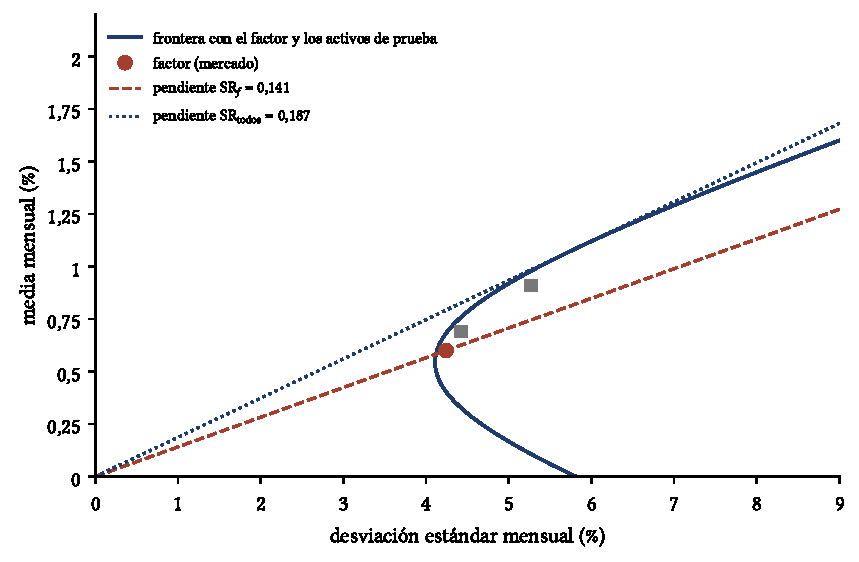
\includegraphics[width=0.72\linewidth]{graficos/cap14_fig_grs.pdf}
\caption{Geometría de la prueba GRS. Con un factor de razón de Sharpe 0,141 y dos activos de prueba con alfas de 0,25 y
0,15 (cuadrados), la cartera tangente alcanza una razón de Sharpe de 0,187. La diferencia entre los cuadrados de ambas
pendientes es exactamente $\boldsymbol\alpha'\Sigma^{-1}\boldsymbol\alpha=0{,}0149$.}
\label{fig:grs}
\end{figure}

% ---------------------------------------------------------------------
\section{Regresiones de corte transversal: Fama-MacBeth}
% ---------------------------------------------------------------------

Cuando los factores no son rendimientos (por ejemplo, el crecimiento del consumo) o cuando se quiere estimar la prima
de cada riesgo directamente, se usa un enfoque de dos pasos. Fama y MacBeth (1973) proponen:
\begin{enumerate}[leftmargin=*]
  \item Estimar las betas de cada cartera con regresiones de series de tiempo: $\hat{\boldsymbol\beta}_i$.
  \item Cada mes $t$, regresar los $N$ excesos de rendimiento sobre las betas:
        $R_{it}=\gamma_{0t}+\hat{\boldsymbol\beta}_i'\boldsymbol\lambda_t+u_{it}$, y promediar en el tiempo:
        \[
          \hat{\boldsymbol\lambda}=\frac1T\sum_{t=1}^{T}\hat{\boldsymbol\lambda}_t,\qquad
          \widehat{\Var}(\hat{\boldsymbol\lambda})=\frac{1}{T^2}\sum_{t=1}^{T}(\hat{\boldsymbol\lambda}_t-\hat{\boldsymbol\lambda})(\hat{\boldsymbol\lambda}_t-\hat{\boldsymbol\lambda})'.
        \]
\end{enumerate}

\begin{proposicion}[Errores estándar de Fama-MacBeth]\label{prop:fm}
Si los $\hat{\boldsymbol\lambda}_t$ no están correlacionados en el tiempo y tienen la misma varianza $V_\lambda$, entonces
$\Var(\hat{\boldsymbol\lambda})=V_\lambda/T$, y el estimador de la proposición es consistente para ella.
\end{proposicion}

\begin{proof}
El promedio de $T$ vectores no correlacionados con varianza común $V_\lambda$ tiene varianza
\begin{align*}
  \Var\Bigl(\frac1T\sum_t\hat{\boldsymbol\lambda}_t\Bigr) &= \frac{1}{T^2}\sum_t\Var(\hat{\boldsymbol\lambda}_t)\\
                                                         &= \frac{1}{T^2}\,T\,V_\lambda\\
                                                         &= \frac{V_\lambda}{T}.
\end{align*}
La varianza muestral de los $\hat{\boldsymbol\lambda}_t$, dividida entre $T$, estima $V_\lambda/T$ de forma consistente. Su
virtud es que incorpora automáticamente la correlación de corte transversal de los errores entre carteras, que una
regresión agrupada ignoraría.
\end{proof}

\paragraph{El problema de las variables generadas.} Las betas del segundo paso son estimaciones con error, y la fórmula
anterior lo ignora. Shanken (1992) muestra que, con betas estimadas en toda la muestra, la varianza correcta es
\[
  \Var(\hat{\boldsymbol\lambda})=\frac1T\Bigl[(X'X)^{-1}X'\Sigma X(X'X)^{-1}\bigl(1+\boldsymbol\lambda'\Omega^{-1}\boldsymbol\lambda\bigr)+\Omega^*\Bigr],
\]
donde $X=(\boldsymbol\iota,\hat B)$ y $\Omega^*$ es la covarianza de los factores bordeada con ceros en la fila y la
columna de la constante. El término $1+\boldsymbol\lambda'\Omega^{-1}\boldsymbol\lambda$ es el mismo que en la
Proposición~\ref{prop:alfas}. Con datos mensuales es pequeño (las razones de Sharpe mensuales lo son), y la corrección
suele cambiar poco los resultados, pero con factores no negociables puede ser grande.

\paragraph{¿Qué mide el $R^2$ de corte transversal?} El ajuste del modelo se juzga comparando los rendimientos promedio
realizados con los ajustados, $\hat\gamma_0+\hat{\boldsymbol\beta}_i'\hat{\boldsymbol\lambda}$. Lewellen, Nagel y Shanken (2010)
advierten que con carteras que tienen una fuerte estructura factorial (como las de tamaño y valor) casi cualquier
factor correlacionado con SMB y HML produce un $R^2$ alto, y recomiendan usar carteras de prueba diversas, como haremos.

% ---------------------------------------------------------------------
\section{Factores estadísticos}
% ---------------------------------------------------------------------

En lugar de proponer factores, pueden extraerse de los datos. Los \emph{componentes principales} de la matriz de
covarianzas $V$ de los rendimientos son las combinaciones lineales $\mathbf v_k'\mathbf R_t$ con los autovectores
$\mathbf v_k$ de $V$, ordenados por su autovalor $\ell_k$. El primero es la combinación de varianza máxima con
$\|\mathbf v\|=1$; el segundo, la de varianza máxima entre las ortogonales al primero, y así sucesivamente. La fracción
$\ell_k/\sum_j\ell_j$ es la parte de la varianza total que explica el componente $k$. La teoría de valoración por
arbitraje (Ross, 1976) justifica que los factores que explican la covarianza sean los que tienen prima; Kozak, Nagel y
Santosh (2018) muestran que los primeros componentes de muchas carteras capturan la mayoría de las anomalías.

% ---------------------------------------------------------------------
\section{Ejercicios resueltos}
% ---------------------------------------------------------------------

\begin{ejresuelto}{CAPM frente a Fama-French}\label{ej:ff3}
\enunciado Estime el CAPM y el modelo de tres factores de Fama y French para las 9 carteras de tamaño y valor.
Compare los alfas y los $R^2$, y la capacidad de cada modelo para explicar la diferencia de rendimiento entre las
acciones pequeñas de valor (S1V5) y las de crecimiento (S1V1).

\solucion
\paso{Paso 1. Resultados.}
\begin{center}\small
\begin{tabular}{@{}lrrrrrrr@{}}
\toprule
 & & \multicolumn{3}{c}{CAPM} & \multicolumn{3}{c}{FF3} \\
\cmidrule(lr){3-5}\cmidrule(lr){6-8}
Cartera & Media & $\hat\alpha$ & $t$ & $R^2$ & $\hat\alpha$ & $t$ & $R^2$ \\
\midrule
S1V1 & 0,344 & $-0{,}547$ & $-3{,}17$ & 0,59 & $-0{,}533$ & $-5{,}14$ & 0,86 \\
S1V3 & 0,833 & 0,137 & 1,17 & 0,65 & $-0{,}049$ & $-0{,}93$ & 0,93 \\
S1V5 & 1,155 & 0,470 & 3,75 & 0,62 & 0,120 & 2,52 & 0,95 \\
S3V1 & 0,625 & $-0{,}200$ & $-1{,}98$ & 0,78 & $-0{,}056$ & $-1{,}08$ & 0,94 \\
S3V3 & 0,839 & 0,190 & 2,56 & 0,80 & 0,006 & 0,11 & 0,90 \\
S3V5 & 1,082 & 0,393 & 3,60 & 0,68 & 0,009 & 0,15 & 0,90 \\
S5V1 & 0,611 & $-0{,}029$ & $-0{,}55$ & 0,89 & 0,136 & 3,57 & 0,94 \\
S5V3 & 0,726 & 0,175 & 2,52 & 0,77 & 0,060 & 1,02 & 0,84 \\
S5V5 & 0,802 & 0,162 & 1,44 & 0,64 & $-0{,}196$ & $-2{,}44$ & 0,82 \\
\bottomrule
\end{tabular}
\end{center}
El promedio de $|\hat\alpha|$ baja de $0{,}256$ a $0{,}129$\,\% mensual y los $R^2$ suben de un rango de 0,59--0,89 a uno de
0,82--0,95. Las cargas en HML van de $-0{,}41$ (crecimiento) a $0{,}84$ (valor), y las de SMB de $-0{,}25$ (grandes) a $1{,}40$
(pequeñas): los factores capturan exactamente las dimensiones con las que se formaron las carteras.

\paso{Paso 2. El diferencial valor-crecimiento.} Las acciones pequeñas de valor rindieron $0{,}811$\,\% mensual más que las de
crecimiento. El CAPM no lo explica; al contrario, como S1V1 tiene más beta (1,38 frente a 1,06), predice que debería rendir
más, y la diferencia de alfas, $0{,}470-(-0{,}547)=1{,}017$, es mayor que la de medias. Con FF3 la diferencia de alfas baja a
$0{,}653$: el modelo explica una parte, pero las acciones pequeñas de crecimiento siguen siendo un caso problemático, con un
alfa de $-0{,}53$\,\% mensual ($t=-5{,}14$), un conocido rompecabezas de la literatura (Figura~\ref{fig:ff3}).

\codigoweb{cap14_ej01}
\salidaR{cap14_ej01_R.txt}
\lectura{cap14_ej01}

\RvsPy Las regresiones de las nueve carteras se resuelven a la vez con un solo sistema $(X'X)B=X'R$, donde cada columna
de $R$ es una cartera; es más rápido y más claro que un bucle de \texttt{lm}. Los excesos de rendimiento se calculan
restando la tasa libre de riesgo, que viene en la misma base: \texttt{as.matrix(...) - f\$RF} en R aprovecha que restar un
vector a una matriz opera por columnas.

\begin{figure}[ht]
\centering
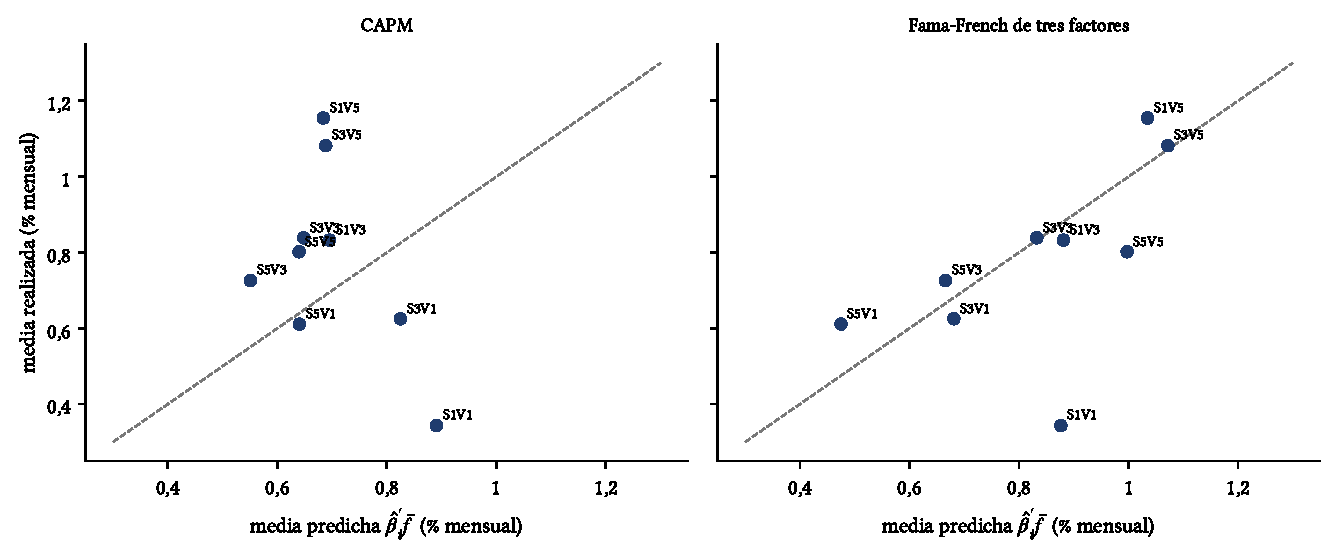
\includegraphics[width=\linewidth]{graficos/cap14_ej01_predicho.pdf}
\caption{Rendimiento medio realizado frente al predicho por cada modelo para las 9 carteras de tamaño y valor. Con un
modelo perfecto, los puntos estarían sobre la diagonal.}
\label{fig:ff3}
\end{figure}

\begin{conclusion}
El modelo de tres factores mejora mucho al CAPM en las carteras de tamaño y valor: reduce los alfas a la mitad y explica
la mayor parte del efecto valor. Pero no lo explica todo, y la cartera de acciones pequeñas de crecimiento sigue lejos
de la diagonal.
\end{conclusion}
\end{ejresuelto}

\begin{ejresuelto}{La prueba GRS}\label{ej:grs}
\enunciado Aplique la prueba GRS al CAPM, al modelo de tres factores y al de cuatro factores de Carhart, con tres conjuntos
de carteras de prueba: tamaño y valor, tamaño y momentum, e industrias.

\solucion
\paso{Paso 1. Resultados.}
\begin{center}\small
\begin{tabular}{@{}llrrr@{}}
\toprule
Carteras & Modelo & $J_{\text{GRS}}$ & Valor $p$ & $|\hat\alpha|$ medio \\
\midrule
Tamaño y valor (9) & CAPM & 7,753 & $5\times10^{-11}$ & 0,256 \\
 & FF3 & 5,754 & $9\times10^{-8}$ & 0,129 \\
 & Carhart & 4,707 & $4\times10^{-6}$ & 0,115 \\
Tamaño y momentum (9) & CAPM & 13,651 & $1\times10^{-20}$ & 0,413 \\
 & FF3 & 12,706 & $5\times10^{-19}$ & 0,425 \\
 & Carhart & 7,858 & $4\times10^{-11}$ & 0,135 \\
Industrias (12) & CAPM & 2,672 & 0,0016 & 0,122 \\
 & FF3 & 5,183 & $2\times10^{-8}$ & 0,167 \\
 & Carhart & 5,082 & $3\times10^{-8}$ & 0,141 \\
\bottomrule
\end{tabular}
\end{center}

\paso{Paso 2. Cálculo para FF3 en tamaño y valor.} Con $T=819$, $N=9$, $L=3$, $\mathrm{SR}^2_f=0{,}05158$ y
$\hat{\boldsymbol\alpha}'\hat\Sigma_{\text{MV}}^{-1}\hat{\boldsymbol\alpha}=0{,}067483$, por la Proposición~\ref{prop:grssharpe}:
\begin{align*}
  J_{\text{GRS}} &= \frac{819-9-3}{9}\cdot\frac{0{,}067483}{1+0{,}05158}\\
                 &= 89{,}667\times0{,}064173\\
                 &= 5{,}754,
\end{align*}
frente a un valor crítico $F_{9,807}$ al 5\,\% de aproximadamente $1{,}89$.

\paso{Paso 3. Interpretación.} Todos los modelos se rechazan con todos los conjuntos: con 69 años de datos la prueba
tiene mucha potencia, y ningún modelo es exactamente cierto. Lo informativo es la comparación. El momentum destruye al
modelo de tres factores: con las carteras de tamaño y momentum, FF3 tiene alfas tan grandes como el CAPM (0,425 frente a
0,413), y solo el factor Mom los reduce a 0,135 (Figura~\ref{fig:alfasmom}). En las industrias, en cambio, agregar SMB y
HML \emph{empeora} el ajuste: los factores de tamaño y valor introducen exposiciones que no se corresponden con
diferencias de rendimiento entre industrias.

\codigoweb{cap14_ej02}
\salidaR{cap14_ej02_R.txt}
\lectura{cap14_ej02}

\RvsPy La matriz $\hat\Omega$ es la covarianza de máxima verosimilitud (dividida entre $T$). En R la calculamos con una
función propia, \texttt{mcov}, porque \texttt{cov} divide entre $T-1$; en Python, \texttt{np.cov(..., bias=True)}. Con un solo
factor, \texttt{np.cov} devuelve un escalar y hay que darle forma de matriz $1\times1$ con \texttt{reshape}.

\begin{figure}[ht]
\centering
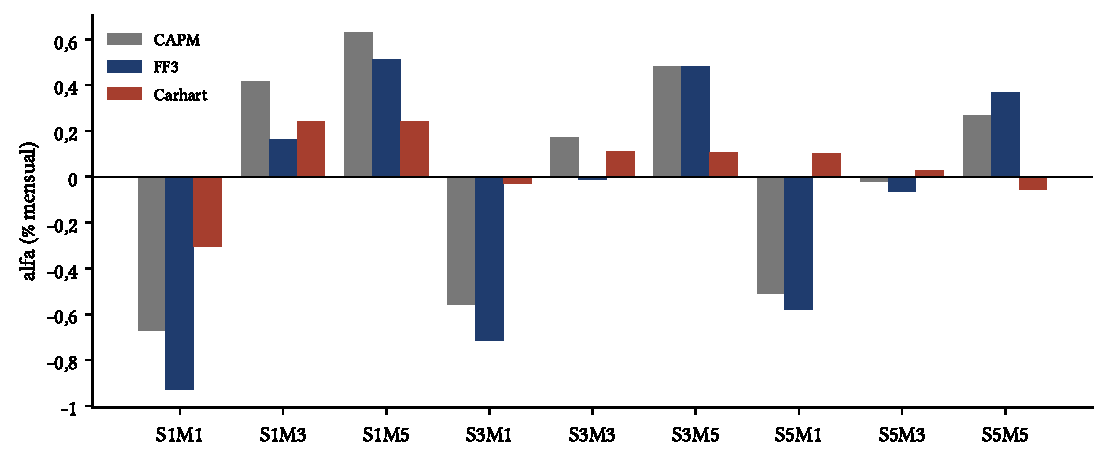
\includegraphics[width=0.88\linewidth]{graficos/cap14_ej02_alfas_momentum.pdf}
\caption{Alfas de las carteras de tamaño y momentum (M1, perdedoras; M5, ganadoras) con cada modelo. Solo el modelo de
Carhart reduce los alfas de las carteras extremas.}
\label{fig:alfasmom}
\end{figure}

\begin{conclusion}
Un modelo de factores debe juzgarse con carteras de prueba que no se hayan formado con sus propias características. El
modelo de tres factores funciona bien donde fue diseñado (tamaño y valor) y mal donde no (momentum, industrias).
\end{conclusion}
\end{ejresuelto}

\begin{ejresuelto}{Primas por riesgo de Fama-MacBeth}\label{ej:fm}
\enunciado Con las 30 carteras, estime las primas por riesgo de los modelos FF3 y Carhart por Fama-MacBeth, con errores
estándar ingenuos y corregidos de Shanken. Compare las primas con las medias de los factores.

\solucion
\paso{Paso 1. FF3.}
\begin{center}\small
\begin{tabular}{@{}lrrrr@{}}
\toprule
 & $\hat\lambda$ & $t$ FM & $t$ Shanken & Media del factor \\
\midrule
Constante & 1,353 & 6,94 & 6,82 & -- \\
Mkt & $-0{,}665$ & $-2{,}70$ & $-2{,}67$ & 0,645 \\
SMB & 0,133 & 1,26 & 1,26 & 0,159 \\
HML & 0,093 & 0,89 & 0,88 & 0,348 \\
\bottomrule
\end{tabular}
\end{center}
El resultado es el contrario del esperado: una constante de 1,35\,\% mensual y una prima de mercado \emph{negativa}, con un
$R^2$ de corte transversal de apenas 0,16. Es el patrón clásico de una línea del mercado de valores demasiado plana:
en el corte transversal, las carteras de más beta no rinden más (Black, Jensen y Scholes, 1972). Si el modelo fuera
correcto, la constante sería cero y cada $\lambda$ igual a la media de su factor.

\paso{Paso 2. Carhart.}
\begin{center}\small
\begin{tabular}{@{}lrrrr@{}}
\toprule
 & $\hat\lambda$ & $t$ FM & $t$ Shanken & Media del factor \\
\midrule
Constante & 0,571 & 3,14 & 3,03 & -- \\
Mkt & 0,150 & 0,64 & 0,63 & 0,645 \\
SMB & 0,102 & 0,97 & 0,97 & 0,159 \\
HML & 0,269 & 2,61 & 2,60 & 0,348 \\
Mom & 0,787 & 5,59 & 5,58 & 0,698 \\
\bottomrule
\end{tabular}
\end{center}
El $R^2$ sube a 0,71 y las primas de HML y Mom quedan cerca de las medias de sus factores (Figura~\ref{fig:fm}). Pero la
constante sigue siendo significativa y la prima de mercado, pequeña.

\paso{Paso 3. La corrección de Shanken.} El término de corrección es $1+\hat{\boldsymbol\lambda}'\hat\Omega^{-1}\hat{\boldsymbol\lambda}=1{,}033$ (FF3) y
$1{,}071$ (Carhart), de modo que los errores estándar de la parte de betas crecen entre 1,6 y 3,5\,\%. Con datos mensuales y
factores negociables la corrección apenas cambia las conclusiones.

\codigoweb{cap14_ej03}
\salidaR{cap14_ej03_R.txt}
\lectura{cap14_ej03}

\RvsPy Las 819 regresiones de corte transversal se resuelven con una sola operación matricial: $(X'X)^{-1}X'R'$ produce una
matriz cuyas columnas son las estimaciones de cada mes. No hace falta ningún bucle. En Python, \texttt{linearmodels} tiene la
clase \texttt{FamaMacBeth}, pero para datos de panel de acciones individuales; para carteras es más transparente
programarlo.

\begin{figure}[ht]
\centering
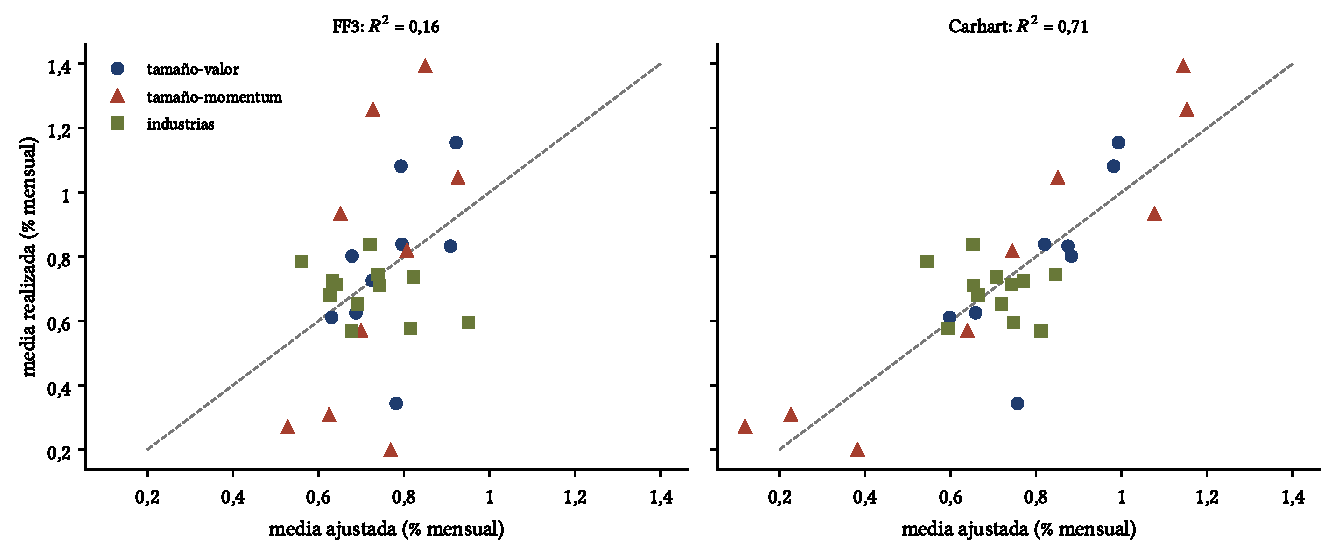
\includegraphics[width=\linewidth]{graficos/cap14_ej03_fama_macbeth.pdf}
\caption{Rendimiento medio realizado frente al ajustado por la regresión de corte transversal, con los modelos FF3 y Carhart,
para las 30 carteras.}
\label{fig:fm}
\end{figure}

\begin{conclusion}
Con carteras de prueba diversas, el modelo de tres factores explica poco del corte transversal de rendimientos; agregar el
momentum lo mejora mucho. La prima de mercado estimada en el corte transversal es casi siempre menor que la del mercado en
el tiempo: las betas altas no se pagan como predice el CAPM.
\end{conclusion}
\end{ejresuelto}

\begin{ejresuelto}{La GRS como razones de Sharpe}\label{ej:grssharpe}
\enunciado Para las 9 carteras de tamaño y valor, verifique numéricamente la Proposición~\ref{prop:grssharpe} con los tres
modelos y compare las razones de Sharpe máximas anuales.

\solucion
\paso{Paso 1. Verificación.} Con el CAPM, la razón de Sharpe mensual del mercado es $0{,}1523$ y la máxima con el mercado y
las 9 carteras, $0{,}3338$:
\begin{align*}
  \mathrm{SR}^2_{\text{todos}}-\mathrm{SR}^2_f &= 0{,}3338^2-0{,}1523^2\\
                                                &= 0{,}11142-0{,}02320\\
                                                &= 0{,}08822\approx0{,}088249,
\end{align*}
que coincide (con todas las decimales en la salida) con $\hat{\boldsymbol\alpha}'\hat\Sigma_{\text{MV}}^{-1}\hat{\boldsymbol\alpha}$. Lo mismo ocurre con FF3
($0{,}067483$) y Carhart ($0{,}058279$).

\paso{Paso 2. Razones de Sharpe anuales.} Multiplicando por $\sqrt{12}$:
\begin{center}\small
\begin{tabular}{@{}lrr@{}}
\toprule
Modelo & Solo factores & Factores y 9 carteras \\
\midrule
CAPM    & 0,528 & 1,156 \\
FF3     & 0,787 & 1,195 \\
Carhart & 1,143 & 1,417 \\
\bottomrule
\end{tabular}
\end{center}
Agregar factores acerca la frontera de los factores a la de todos los activos, pero la brecha nunca se cierra
(Figura~\ref{fig:sharpe}). Por separado, el factor de mayor razón de Sharpe mensual es Mom ($0{,}179$), seguido del mercado
($0{,}152$), HML ($0{,}129$) y SMB ($0{,}056$).

\codigoweb{cap14_ej04}
\salidaR{cap14_ej04_R.txt}
\lectura{cap14_ej04}

\RvsPy La identidad es exacta en la muestra solo si las covarianzas se calculan dividiendo entre $T$; con la covarianza
insesgada habría una discrepancia en la cuarta cifra. En ambos lenguajes, $\mathbf m'V^{-1}\mathbf m$ se calcula con
\texttt{solve} en lugar de invertir $V$, que es más estable numéricamente.

\begin{figure}[ht]
\centering
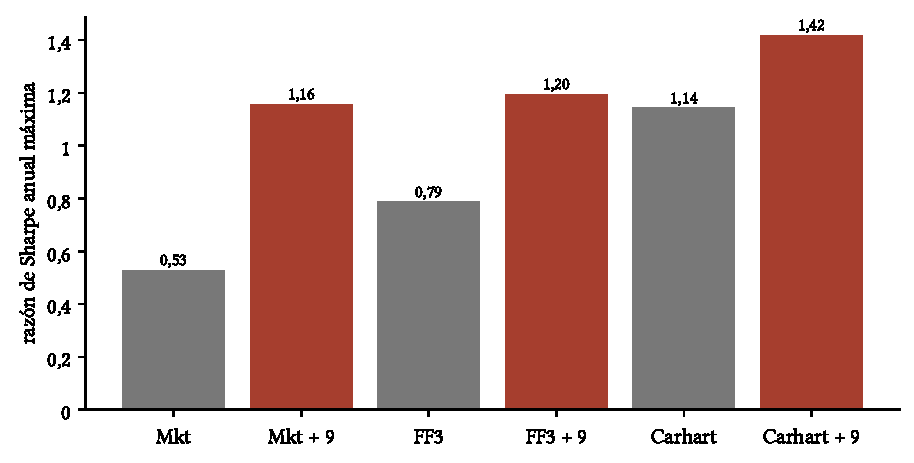
\includegraphics[width=0.72\linewidth]{graficos/cap14_ej04_sharpe.pdf}
\caption{Razón de Sharpe anual máxima con cada conjunto de factores (gris) y al agregar las 9 carteras de tamaño y valor
(rojo). La diferencia de los cuadrados es lo que mide la prueba GRS.}
\label{fig:sharpe}
\end{figure}

\begin{conclusion}
Rechazar un modelo con la prueba GRS significa que existe una cartera de los activos de prueba que mejora la razón de
Sharpe de los factores. En estos datos, la mejora es grande para el CAPM (de 0,53 a 1,16 anual) y menor, pero aún
significativa, para el modelo de Carhart.
\end{conclusion}
\end{ejresuelto}

\begin{ejresuelto}{Componentes principales}\label{ej:pca}
\enunciado Extraiga los componentes principales de la matriz de covarianzas de las 30 carteras. ¿Qué parte de la varianza
explican? ¿Con qué factores se relacionan los tres primeros?

\solucion
\paso{Paso 1. Varianza explicada.} El primer componente explica el 73,46\,\% de la varianza total; el segundo, el 6,29\,\%; el
tercero, el 4,01\,\%. Los tres primeros, el 83,76\,\%. Hay una fuerte estructura factorial: un solo factor domina.

\paso{Paso 2. Interpretación.}
\begin{center}\small
\begin{tabular}{@{}lrrrrr@{}}
\toprule
 & Mkt & SMB & HML & Mom & $R^2$ con los cuatro \\
\midrule
CP1 & 0,962 & 0,462 & $-0{,}128$ & $-0{,}206$ & 0,989 \\
CP2 & 0,217 & $-0{,}801$ & 0,056 & 0,010 & 0,836 \\
CP3 & 0,107 & 0,094 & $-0{,}562$ & 0,855 & 0,916 \\
\bottomrule
\end{tabular}
\end{center}
El primer componente es casi el mercado (correlación 0,96; todas las cargas positivas). El segundo es un factor de tamaño,
con signo opuesto a SMB: contrapone acciones grandes y pequeñas. El tercero mezcla momentum y valor con signos opuestos, lo
que refleja la conocida correlación negativa entre ambas estrategias (Figura~\ref{fig:pca}).

\paso{Paso 3. Ajuste.} Tres componentes producen un $R^2$ medio de series de tiempo de 0,817 en las 30 carteras, algo más que
Mkt, SMB y HML (0,794). Los componentes están diseñados para explicar la covarianza; no garantizan explicar los
\emph{rendimientos medios}, que es lo que importa para la valoración.

\codigoweb{cap14_ej05}
\salidaR{cap14_ej05_R.txt}
\lectura{cap14_ej05}

\RvsPy El signo de un autovector es arbitrario: \texttt{eigen} de R y \texttt{np.linalg.eigh} de Python pueden devolver
signos opuestos. Para que los resultados coincidan, normalizamos cada autovector para que la suma de sus cargas sea
positiva. Además, \texttt{eigh} ordena los autovalores de menor a mayor y \texttt{eigen} de mayor a menor.

\begin{figure}[ht]
\centering
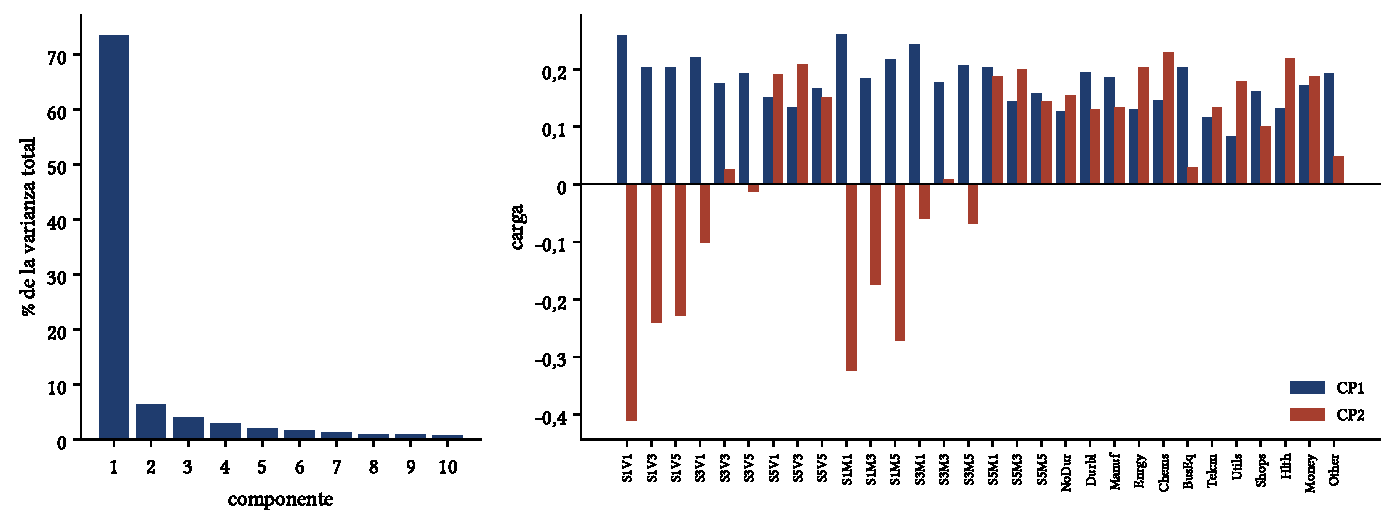
\includegraphics[width=\linewidth]{graficos/cap14_ej05_componentes.pdf}
\caption{Izquierda: fracción de la varianza explicada por los diez primeros componentes. Derecha: cargas de los dos primeros
componentes en las 30 carteras; el primero carga positivamente en todas y el segundo separa pequeñas de grandes.}
\label{fig:pca}
\end{figure}

\begin{conclusion}
Los datos encuentran por sí solos un factor de mercado y uno de tamaño, y un tercero relacionado con momentum y valor. Los
factores económicos de Fama, French y Carhart son, en buena medida, rotaciones de los factores estadísticos dominantes.
\end{conclusion}
\end{ejresuelto}

% ---------------------------------------------------------------------
\section{Ejercicios propuestos}
% ---------------------------------------------------------------------

\begin{enumerate}[label=\textbf{\thechapter.\arabic*},leftmargin=*,itemsep=6pt]
  \item Con $T=600$, $N=25$, $L=3$, $\mathrm{SR}^2_f=0{,}04$ y $\hat{\boldsymbol\alpha}'\hat\Sigma_{\text{MV}}^{-1}\hat{\boldsymbol\alpha}=0{,}06$, calcule el
  estadístico GRS. \textit{Respuesta: $1{,}320$.}

  \item Demuestre que, en el CAPM con un solo factor, $1+\mathrm{SR}^2_f=1+\bar f^2/\hat\sigma_f^2$ y que el error estándar del alfa
  es $\hat\sigma_\varepsilon\sqrt{(1+\bar f^2/\hat\sigma_f^2)/T}$.

  \item Verifique que $V=GDG'$ en la demostración de la Proposición~\ref{prop:grssharpe}.

  \item Demuestre que el primer componente principal maximiza $\mathbf v'V\mathbf v$ sujeto a $\mathbf v'\mathbf v=1$ y que el
  máximo es el mayor autovalor de $V$.

  \item ¿Por qué un factor negociable debe tener una prima igual a su media? (Sugerencia: aplique el modelo al propio factor.)

  \item \emph{(Simulación.)} Simule 1\,000 muestras de $T=240$ meses de 10 carteras que cumplen exactamente el CAPM, con betas
  entre 0,5 y 1,5. Calcule la frecuencia de rechazos de la GRS al 5\,\% y de al menos un $t$ individual mayor que 1,96. ¿Por
  qué difieren?

  \item \emph{(Con datos de Yahoo Finance.)} Forme carteras de acciones de la Bolsa de Valores de Lima por tamaño y estime el
  CAPM con el índice S\&P/BVL Perú General como mercado. ¿Hay efecto tamaño en el mercado peruano?

  \item \emph{(Con datos.)} Divida la muestra en 1949--1983 y 1984--2017 y repita el Ejercicio~\ref{ej:fm}. ¿Es estable la prima de
  momentum?
\end{enumerate}

% ---------------------------------------------------------------------
\section{Resumen de fórmulas}
% ---------------------------------------------------------------------

\begin{table}[H]
\centering\small
\begin{tabular}{@{}ll@{}}
\toprule
Concepto & Fórmula \\
\midrule
Modelo de series de tiempo & $R_{it}=\alpha_i+\boldsymbol\beta_i'\mathbf f_t+\varepsilon_{it}$;\quad $H_0$: $\boldsymbol\alpha=\mathbf 0$ \\
Varianza de los alfas & $(1+\hat{\boldsymbol\mu}'\hat\Omega^{-1}\hat{\boldsymbol\mu})\Sigma/T$ \\
GRS & $\frac{T-N-L}{N}\frac{T}{T-L-1}\frac{\hat{\boldsymbol\alpha}'\hat\Sigma^{-1}\hat{\boldsymbol\alpha}}{1+\hat{\boldsymbol\mu}'\hat\Omega^{-1}\hat{\boldsymbol\mu}}\sim F_{N,T-N-L}$ \\
GRS y Sharpe & $\hat{\boldsymbol\alpha}'\hat\Sigma_{\text{MV}}^{-1}\hat{\boldsymbol\alpha}=\mathrm{SR}^2_{\text{todos}}-\mathrm{SR}^2_f$ \\
Fama-MacBeth & $\hat{\boldsymbol\lambda}=\frac1T\sum_t\hat{\boldsymbol\lambda}_t$;\quad $\widehat{\Var}=\frac{1}{T^2}\sum_t(\hat{\boldsymbol\lambda}_t-\hat{\boldsymbol\lambda})(\cdot)'$ \\
Shanken & $\frac1T[(X'X)^{-1}X'\Sigma X(X'X)^{-1}(1+\boldsymbol\lambda'\Omega^{-1}\boldsymbol\lambda)+\Omega^*]$ \\
Componentes principales & $V\mathbf v_k=\ell_k\mathbf v_k$;\quad varianza explicada $\ell_k/\sum_j\ell_j$ \\
\bottomrule
\end{tabular}
\caption{Fórmulas principales del Capítulo 14.}
\end{table}

\section*{Referencias}
\begin{itemize}[leftmargin=*]
  \item Black, F., Jensen, M. C. y Scholes, M. (1972). The capital asset pricing model: Some empirical tests. En M. C. Jensen
        (ed.), \emph{Studies in the Theory of Capital Markets}, 79--121. Praeger.
  \item Carhart, M. M. (1997). On persistence in mutual fund performance. \emph{Journal of Finance}, 52(1), 57--82.
  \item Cochrane, J. H. (2005). \emph{Asset Pricing}, ed. revisada. Princeton University Press.
  \item Fama, E. F. y French, K. R. (1993). Common risk factors in the returns on stocks and bonds. \emph{Journal of Financial
        Economics}, 33(1), 3--56.
  \item Fama, E. F. y MacBeth, J. D. (1973). Risk, return, and equilibrium: Empirical tests. \emph{Journal of Political
        Economy}, 81(3), 607--636.
  \item Gibbons, M. R., Ross, S. A. y Shanken, J. (1989). A test of the efficiency of a given portfolio. \emph{Econometrica},
        57(5), 1121--1152.
  \item Kozak, S., Nagel, S. y Santosh, S. (2018). Interpreting factor models. \emph{Journal of Finance}, 73(3), 1183--1223.
  \item Lewellen, J., Nagel, S. y Shanken, J. (2010). A skeptical appraisal of asset pricing tests. \emph{Journal of Financial
        Economics}, 96(2), 175--194.
  \item Ross, S. A. (1976). The arbitrage theory of capital asset pricing. \emph{Journal of Economic Theory}, 13(3), 341--360.
  \item Shanken, J. (1992). On the estimation of beta-pricing models. \emph{Review of Financial Studies}, 5(1), 1--33.
\end{itemize}
